\section{基于 BIM 的规则检查}
\subsection{规则检查方法}
现有的安全规则、指南和最佳实践可以与现有的三维 (3D) 设计和进度
信息结合使用,以形成一个自动化的安全规则检查系统。其目的是在建
筑物建造时自动识别这些动态条件,在虚拟 3D 空间中识别它们的位置,
并交互式或自动地为多种危险提供解决方案和保护系统的可视
化。

这个平台可以作为一种工具,使人们能够方便地、易于理解地
看到随着时间的推移在建筑和安全方面取得的最新进展,特别是能够发
现工地上的危险地点。安全措施的指示将有助于安全管理人员在施工计
划阶段以及施工期间提前规划安全。规则检查程序包括以下程序:

\begin{itemize}
    \item 规则解释:从安全规则或最佳实践(例如,OSHA) 对安全规则的解
    释是一个基于逻辑的映射,从人类语言到机器可读的形式。可
    以从书面规则中分析和提取规则中的名称、类型和其他属性。
    构建模型准备:必须很好地构建构建模型,以包括用于进行规则
    检查的所需对象、属性和关系。此外,由于防堕设备的需要取
    决于施工工作的状况,因此需要一个包括建筑组件安装时间表/
    顺序的 4D模型。
    \item 规则执行:规则执行阶段将转换后的规则集与准备好的构建模型
    集合在一起。该规则可应用于数以千计的条件情形,需要组合
    跟踪。规则的执行有两个步骤:(a) 自动检查模型以识别不安全的
    条件,(b) 识别和应用候选解决方案
    \item 纠正不安全情况的行动。这最后一步可以通过多种方式控制,
    对每种情况进行人工干预,通过应用规则来确定最佳修正,从
    而完全自动地解决问题。
    \item 规则检查报告:检查结果可以以多种形式报告:(a) 使模型中应用的
    安全防护设备可视化,(b) 基于 excel 的不安全状况报告和采取的
    纠正措施。此外,为安全设备的资源平衡和将生成的信息导入
    项目进度表提供数量启动信息也是可能的。
    \item 安全纠正:在建筑工地上采取的主要纠正措施是根据规则检查报
    告安排和跟踪(安全)材料的后勤运输。例如,一个现场的实现可
    以是在 BIM 平台上报告,该平台为建筑楼层安装和拆除安全设
    备分配工作任务。
    \item 这是对规则检查系统一般需求的扩展,包括了安全改进步骤。
\end{itemize}

\subsection{基于规则的算法在案例研究中的应用}

一旦建立了良好的建筑物信息模型,并且建立了模型对象与调度之
间的联系,就可以应用规则进行安全隐患的检测。 Zhang 给出了如下的解释方法:

\begin{enumerate}
    \item 板坯边缘保护:图 \ref{fig:c3f1} 解释了根据 OSHA 安全规则检测所需预防方法的算法
    对于每个任务,它检查 slab 对象是否链接到给定的工作任务。对
    于与任务相关联的每个 slab 对象,该算法检查 slab 是否需要与现
    有的 slab 合并。如果在同一水平面上没有现有的板,则计算板边
    界。此外,现有的墙壁膨胀检测,看看是否有任何部分的板边界
    不需要下降保护。因此,无保护的边缘需要护栏保护计算。另外,
    根据平板合并后的几何条件分别计算存在边、未保护边和重叠边。
    因此,新的护栏安装没有保护的边缘和现有的护栏重叠的边缘被
    删除。
    \item 板坯孔保护:一般有两种方法检测板坯孔洞:基于几何的检测和基于对象的检测。由于某些孔洞
    是设计人员为建立复杂的板几何模型而切割的,因此不应将其归
    类为潜在落差孔洞。因此,即使基于几何的检测可以找到所有的
    内部多边形的板,这些将包括一些假阳性错误。对于基于对象的
    检测,它需要额外的标记努力,以协助从模型中的其他空洞对象
    的孔识别。在这项研究中,我们主要依靠基于物体的目标识别,
    但也通过比较板的深度和孔的深度来检查是否是一个会产生坠落
    危险的直通孔。理想情况下,为了清楚地区分这两种情况,在建
    模阶段,工程师应该有两种不同的工具/按钮来 (a) 为复杂几何和
     (b) 为实际切割平板而切割。
    \item 墙体开孔保护:墙体开孔检测过程类似于板坯孔检测。要考虑的特殊
    情况是墙元件的位置:它是内墙还是外墙。对于那些位于板的边缘
    的,一旦墙元素已经安装完毕后,可以拆除板坯边缘保护的护栏,同时,如果存在墙
    口需要进行保护。如果在靠近内墙的地方没有板孔(例如电梯井的
    孔),则不需要考虑或保护墙开口。
\end{enumerate}

\begin{figure}[thbp!]
    \centering
    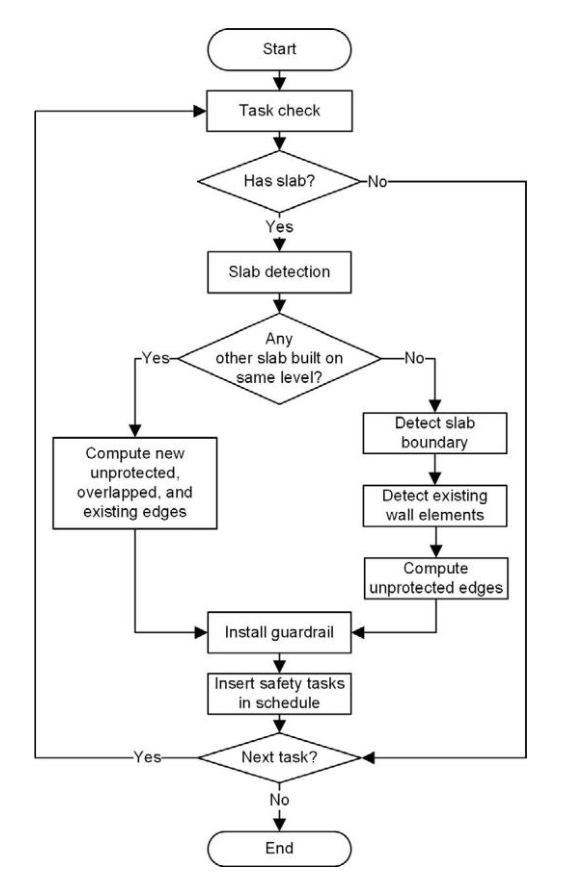
\includegraphics[width=1.0\linewidth]{res/c3f1.png}
    \caption{检测板坯边缘所需预防措施的规则检查算法}
    \label{fig:c3f1}
\end{figure}




